\documentclass[10pt,twocolumn,letterpaper]{article}
\usepackage[pagenumbers]{cvpr}
\usepackage{microtype}
\usepackage{mathtools}
\usepackage{tikz}
\usetikzlibrary{positioning,arrows.meta,fit,calc}
\definecolor{linkblue}{RGB}{28,79,124}
\usepackage[pagebackref,breaklinks,colorlinks,allcolors=linkblue]{hyperref}
\hypersetup{pdftitle={Regenerative Autoencoders: Learning Spatial Structure in a Single Astronomical Image},pdfauthor={Alejandro Hernandez Ruiz}}
\hfuzz=0pt
\vfuzz=0pt
\hbadness=1000
\vbadness=1000

\title{Regenerative Autoencoders:\\Learning Spatial Structure in a Single Astronomical Image}
\author{Alejandro Hernandez Ruiz\\
  {\small First draft, version 0.1 --- October 18, 2026}}

\begin{document}
% Explicit English hyphenation minima for portable TeX formats.
\lefthyphenmin=2
\righthyphenmin=3
\maketitle

\begin{abstract}
Learning the appearance of small image patches does not determine how those patches are arranged. We investigate this distinction with Regenerative Autoencoders (ReGAE), a two-level architecture trained on a single large astronomical image. A patch encoder and conditional denoising decoder first learn local appearance. A second denoiser, called the Gencoder, uses the same architecture family to predict spatial windows of patch representations. Its target is encoded on a fractionally displaced image grid, so prediction changes the pixel support of every latent location rather than merely extending a border. Recurrent evaluation on overlapping windows provides a mechanism for generating and traversing larger image regions without global coordinate conditioning. We describe an implementation using $32\times32$ RGB patches, 256-dimensional codes, and $32\times32$ latent windows, corresponding to approximately megapixel image regions. The case study uses a 236.8-megapixel James Webb Space Telescope mosaic of Pandora's Cluster. Archived training traces support optimization of both stages; historical qualitative observations motivate a discussion of coherent structure, noisy rendering, and transitions between visually ambiguous regions. We relate the construction to diffusion autoencoders, denoising dynamics, and hierarchical compression, while distinguishing these connections from established score-model or continuous-time equivalences. This exploratory report documents the architecture and existing evidence without adding new experiments.
\end{abstract}

\section{Introduction}
\label{sec:introduction}

Generation constructs a sample from an initial state; repair resumes that construction after the sample has been disturbed. The term \emph{regeneration} comes here from the biological motivation of neural cellular automata. Growing NCA distinguishes growth from a seed, persistence of the resulting pattern, and recovery after damage~\cite{nca}. We adopt regeneration in this behavioral sense, rather than as a separate category of probabilistic model or a capability exclusive to cellular automata.

Neural Cellular Automata Manifold (NCAM) supplies the autoencoding lineage: an encoder selects a cellular growth program capable of reconstructing a target image~\cite{ncam}. Regenerative Autoencoders (ReGAE) retain the idea of a reusable reconstruction process while replacing the cellular decoder with a shape-preserving denoiser. The denoiser acts on a corrupted version of the desired state and directly predicts a corrected state. Its output becomes the input to the next update. Starting with noise gives generation; starting with a disturbed reconstruction gives regeneration. In the conditional form, a latent code identifies the intended reconstruction throughout either process.

Neither an iteration index nor a corruption-strength label is supplied to the ReGAE denoiser. At fixed conditioning, the same state is therefore handled by the same learned map wherever it occurs in a trajectory. This motivates viewing generation and repair as movement under one correction field, learned across a range of corruptions. The interpretation is related to diffusion and flow models, but their prediction targets, dependence on time, and sampling rules need to be separated carefully. A single map does not by itself establish a scalar optimization landscape or a globally attracting solution.

\begin{figure*}[t]
  \centering
  % TikZ fragment for a full-width figure. Requires tikz and arrows.meta.
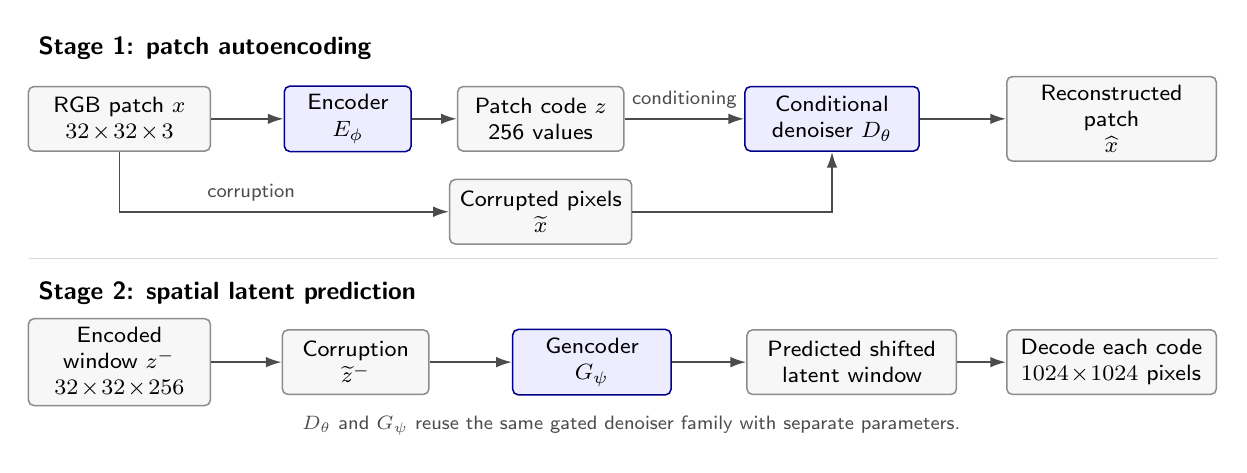
\begin{tikzpicture}[
  x=1cm,y=1cm,
  font=\sffamily\footnotesize,
  >={Latex[length=2mm,width=1.35mm]},
  box/.style={draw=black!45,rounded corners=2pt,line width=.55pt,
              fill=black!3,align=center,minimum height=.82cm,inner sep=3pt},
  net/.style={box,draw=blue!55!black,fill=blue!7},
  flow/.style={->,line width=.65pt,draw=black!70},
  note/.style={font=\sffamily\scriptsize,text=black!70,align=center}
]
% Pixel-level reconstruction.
\node[anchor=west,font=\sffamily\bfseries\small] at (-.1,1.55)
  {Stage 1: patch autoencoding};
\node[box,text width=2.1cm] (rgb) at (1.05,.65)
  {RGB patch $x$\\$32\!\times\!32\!\times\!3$};
\node[net,text width=1.4cm] (enc) at (3.95,.65)
  {Encoder\\$E_{\phi}$};
\node[box,text width=1.9cm] (code) at (6.4,.65)
  {Patch code $z$\\256 values};
\node[net,text width=2.0cm] (dec) at (10.1,.65)
  {Conditional\\denoiser $D_{\theta}$};
\node[box,text width=2.45cm] (recon) at (13.65,.65)
  {Reconstructed patch\\$\widehat{x}$};
\node[box,text width=2.1cm] (corruptx) at (6.4,-.53)
  {Corrupted pixels\\$\widetilde{x}$};
\draw[flow] (rgb)--(enc);
\draw[flow] (enc)--(code);
\draw[flow] (code)--node[note,above]{conditioning}(dec);
\draw[flow] (dec)--(recon);
\draw[flow] (rgb.south) |- node[note,pos=.70,above]{corruption} (corruptx.west);
\draw[flow] (corruptx.east) -| (dec.south);
\draw[black!15,line width=.5pt] (-.1,-1.12)--(15.0,-1.12);
% Spatial latent prediction, followed by patchwise reconstruction.
\node[anchor=west,font=\sffamily\bfseries\small] at (-.1,-1.57)
  {Stage 2: spatial latent prediction};
\node[box,text width=2.1cm] (window) at (1.05,-2.44)
  {Encoded window $z^-$\\$32\!\times\!32\!\times\!256$};
\node[box,text width=1.65cm] (corruptz) at (4.05,-2.44)
  {Corruption\\$\widetilde{z}^-$};
\node[net,text width=1.8cm] (gen) at (7.05,-2.44)
  {Gencoder\\$G_{\psi}$};
\node[box,text width=2.45cm] (shifted) at (10.35,-2.44)
  {Predicted shifted\\latent window};
\node[box,text width=2.45cm] (image) at (13.65,-2.44)
  {Decode each code\\$1024\!\times\!1024$ pixels};
\draw[flow] (window)--(corruptz);
\draw[flow] (corruptz)--(gen);
\draw[flow] (gen)--(shifted);
\draw[flow] (shifted)--(image);
\node[note] at (7.55,-3.25)
  {$D_{\theta}$ and $G_{\psi}$ reuse the same gated denoiser family with separate parameters.};
\end{tikzpicture}

  \caption{Conditional and unconditional members of the ReGAE family. Both denoisers return a state with the same shape as their input, allowing the output to be fed back for successive updates. Generation initializes the state with noise; regeneration re-enters the same loop with a perturbed state. In the conditional model, an encoder supplies a latent tensor that is retained during regeneration. The unconditional model has no encoder-derived conditioning and can model data or learned representations. The two rows illustrate variants, not mandatory levels of one hierarchy.}
  \label{fig:architecture}
\end{figure*}

The broader question motivating this work is what it takes to learn, or \emph{memorize}, a dataset. Calling a model a memorizer does not explain how that memory is organized, which properties it retains, or how it makes them available for generation. A dataset contains information about individual samples and, potentially, relationships among them. Learning to reconstruct a sample addresses one part of this problem. Learning the distribution or organization of its representations addresses another. These are useful questions even before asking whether a system extrapolates beyond its training data.

ReGAE provides a reusable modeling component for investigating those questions. An encoder can concentrate information about a particular sample into a code, while a conditional denoiser learns how to recover the sample from different corrupted states. Removing the encoder and its conditioning pathway gives an unconditional member of the family: a denoiser whose evolving state supplies its context. Such a model can operate directly on data or on representations produced by another model. Conditional and unconditional ReGAE instances can therefore be composed, without requiring a particular number of levels or a particular kind of dataset.

The experiments presented here use a large image of Pandora's Cluster as an example dataset. An image-patch autoencoder learns local appearance, while a second, unconditional ReGAE learns the spatial organization of the resulting patch codes. We call this latent-space instance the \emph{Gencoder}. Predicting codes for a slightly displaced view couples regeneration to a spatial transition. This arrangement is appropriate because spatial relationships are an important part of the information in this dataset. It is an application of the family, rather than its definition.

A different dataset would suggest a different decomposition. For a collection such as CIFAR-10, the first autoencoder could represent each complete image. A subsequent model could learn the distribution of image codes or, with suitable inputs and supervision, relationships between image and class representations. There would be no reason to impose the spatial arrangement used for Pandora's Cluster. This example illustrates the intended scope; it is not an additional experiment reported here.

The defining design choice is thus an iteratively reusable, shape-preserving denoiser, with optional latent conditioning. Its internal architecture, data dimensionality, reconstruction loss, and placement within a hierarchy are configurable. We describe this general construction first, then use the astronomical-image proof of concept to examine the distinction between sample reconstruction and modeling relationships among samples. The discussion connects regeneration to denoising dynamics, architectural reuse, and compression, while keeping the broader proposal distinct from the evidence supplied by the existing experiments.

\section{Related Work}
\label{sec:related}

\paragraph{Regenerative neural dynamics.}
Growing Neural Cellular Automata learn local update rules that develop an image from a seed and can restore a damaged pattern~\cite{nca}.
Neural Cellular Automata Manifold (NCAM) extends this construction to an autoencoding setting, using dynamic convolutions to condition cellular development on an image representation~\cite{ncam}.
ReGAE continues this investigation of learned reconstruction dynamics, with revised conditioning and a denoising objective.
Its U-Net and attention components provide interactions beyond a strictly local cellular rule.
The relevant continuity is therefore the use of learned, repeatedly applicable reconstruction operators, rather than an identical cellular architecture.

\paragraph{Denoising as generative modeling.}
Bengio et al.~\cite{dae} show how alternating corruption and learned denoising can define a generative Markov chain, and introduce walkback training to address spurious modes encountered during sampling.
Alain and Bengio~\cite{alain} connect regularized reconstruction to the score of the data density, including the small-Gaussian-corruption regime.
These results motivate interpreting denoisers as learning local structure around the data distribution.
ReGAE uses a feature-space reconstruction loss, following the broader perceptual-loss approach of Johnson et al.~\cite{perceptual}, with VGG features~\cite{vgg}, and an $L_1$ latent prediction loss.
The score identities derived for particular reconstruction objectives do not directly establish a score interpretation for these losses.

\paragraph{Diffusion and continuous-time models.}
Denoising diffusion probabilistic models connect a prescribed forward noise process to a learned reverse process~\cite{ddpm}.
DDIM constructs non-Markovian processes with the same training objective and permits deterministic sampling~\cite{ddim}.
Score-based SDEs unify several such constructions and yield a probability-flow ODE with matching time-marginal distributions under the corresponding score field~\cite{sde}.
Neural ODEs more generally parameterize a continuous-time derivative and compute trajectories using a differential-equation solver~\cite{neuralode}.
These perspectives suggest useful questions about ReGAE's trajectories, stability, and noise injection.
The implementation studied here defines a discrete denoising map without explicit noise-time conditioning or a learned continuous-time velocity.
Consequently, its recurrent application is a stochastic dynamical system, while identification with a reverse diffusion or probability-flow ODE would require additional assumptions and a derivation.

\paragraph{Autoencoding and latent generative structure.}
Diffusion Autoencoders (DiffAE) are a particularly close comparison~\cite{diffae}.
They combine a learned semantic encoder with a conditional DDIM decoder, representing an image through a 512-dimensional nonspatial semantic vector and a spatial stochastic code.
The latter retains image-specific variations needed for near-exact reconstruction; the semantic vector alone is not the complete code.
DiffAE also learns a latent DDIM prior over semantic vectors for unconditional generation, using a deep multilayer perceptron with skip connections.
Latent diffusion models similarly place generative denoising in the representation space of a pretrained autoencoder~\cite{ldm}.
ReGAE's Gencoder learns relationships across a spatial array of patch representations and predicts the encodings of slightly displaced image patches.
This changes the patch support throughout the target array and couples latent denoising to spatial prediction.
Overlapping recurrent predictions then support image traversal without global coordinate conditioning.
Our focus is this spatial transition mechanism and its integration with regenerative decoding, rather than the general presence of a second latent model.

\paragraph{Learning from a single image.}
SinGAN learns a hierarchy of patch distributions at different scales from one natural image, enabling synthesis that preserves appearance and larger structures~\cite{singan}.
It establishes the importance of multiscale internal image statistics for this setting.
ReGAE studies a related division between local appearance and spatial organization through encoded patches and displaced latent prediction.
The single-image setting makes the distinction between reconstructing a particular arrangement and generating configurations with familiar local content especially visible.

\paragraph{Representation and compression.}
Minimum description length evaluates models through the length of their description together with the data description they support~\cite{mdl}.
COIN provides an operational image-compression example by fitting a coordinate network and storing its quantized weights~\cite{coin}.
Recent work on language-model compression also connects predictive distributions to explicit coding procedures~\cite{lmcompression}.
These perspectives distinguish a low-dimensional representation from a complete compressed bitstream.
ReGAE's hierarchy concerns reusable descriptions of appearance and spatial structure; assessing it as a codec would additionally require accounting for precision, model storage, residual information, and reconstruction distortion.

\section{The ReGAE Model Family}
\label{sec:method}

A conditional Regenerative AutoEncoder (ReGAE) combines a compressed representation with a denoising operator that can be applied repeatedly to a mutable state. The representation specifies what to reconstruct, while the state supplies the current reconstruction, partial observation, or noise initialization. An unconditional member omits the encoder and its conditioning, retaining the recurrent denoiser. We describe these variants independently of the dimensionality, network widths, loss, and sampling choices of the Pandora's Cluster case study.

\subsection{State, encoding, and conditional update}

Let $\mathcal{X}$ be a space of sample tensors and $\mathcal{Z}$ a latent tensor space. An encoder $E_\phi:\mathcal{X}\to\mathcal{Z}$ compresses a sample $x$ into $z=E_\phi(x)$. Neither space has a prescribed dimensionality: the latent may be a vector or a structured tensor, with a bottleneck chosen for the task. Compression here describes the learned representation; its storage cost also depends on numerical precision and model parameters.

The conditional denoiser has the interface
\begin{equation}
  D_\theta:\mathcal{X}\times\mathcal{Z}\to\mathcal{X},
  \qquad x_{t+1}=D_\theta(x_t,z).
  \label{eq:family-recurrence}
\end{equation}
For a chosen configuration, its state input and output have the same dimensions, allowing the output to become the next input without a separate encoding step. The same construction accommodates one-, two-, or three-dimensional state layouts, using suitable operators for sequences, images, or volumetric tensors. This is an architectural interface, rather than a claim that all such domains have been evaluated here.

The latent remains fixed during a conditional trajectory. Parameters are also shared across updates: iteration changes the state, not the learned weights. Conditioning can enter through feature modulation or another compatible mechanism. The encoder is needed to obtain a code from an observed sample; repeated denoising subsequently uses that code directly.

\subsection{Learning a regenerative denoiser}

Training presents a corrupted version of a clean sample and asks the denoiser to recover the sample given its encoding. Let $C_\alpha(x,\epsilon)$ denote a corruption operator, with severity $\alpha$ and random variable $\epsilon$. One useful choice is the mixture
\begin{equation}
  C_\alpha(x,\epsilon)=(1-\alpha)x+\alpha\epsilon,
  \qquad 0\leq\alpha\leq1.
  \label{eq:family-corruption}
\end{equation}
The noise distribution, severity distribution, and any spatial masking are configuration choices. Including both weak and strong corruption connects refinement of an existing state with reconstruction from noise. The conditional training objective is
\begin{equation}
  \mathcal{L}_{\mathrm{cond}}=
  \mathbb{E}_{x,\alpha,\epsilon}\left[
    \ell\bigl(D_\theta(C_\alpha(x,\epsilon),E_\phi(x)),x\bigr)
  \right].
  \label{eq:family-conditional-loss}
\end{equation}
The reconstruction criterion $\ell$ may be an L1 loss, squared L2 loss, or feature-based \emph{perceptive} loss, chosen according to the data and desired fidelity. A feature loss compares representations of the prediction and target; it does not define the ReGAE family. Likewise, a particular noise schedule or optimizer is an implementation choice.

Equation~\eqref{eq:family-conditional-loss} trains an individual restoration step. Repeated application at inference is a separate use of that learned operator. Good one-step reconstruction does not alone establish convergence of every trajectory, preservation of all details, or recovery from arbitrary perturbations. Regeneration must therefore be assessed for the corruption types and update horizons of interest.

\subsection{Generation and regeneration}

Conditional generation starts from a noise state $x_0\sim p_0$ and applies Eq.~\eqref{eq:family-recurrence} for a chosen number of updates. When $z=E_\phi(x)$, this constructs a reconstruction associated with the encoded sample. Generating new samples through new codes additionally requires a way to choose those codes; the conditional autoencoder alone does not specify their prior distribution.

Regeneration uses the same update after an external perturbation. If $\widehat{x}$ is a current reconstruction and $P$ describes damage or corruption, set
\begin{equation}
  y_0=P(\widehat{x}),\qquad
  y_{t+1}=D_\theta(y_t,z).
  \label{eq:family-regeneration}
\end{equation}
The unchanged code supplies a reference while the denoiser acts on the altered state. Noise injection or partial-state refresh between updates can also be used as sampling choices. These interventions change the trajectory without requiring a new encoder evaluation or parameter update. A stable reconstruction may behave as an approximate fixed point, but fixed-point existence, attraction, and universal convergence are not assumed by the definition.

\subsection{Unconditional variant and architecture}

An unconditional ReGAE omits the encoder and external latent code, retaining the state-to-state denoiser:
\begin{equation}
  \begin{aligned}
    x_{t+1}&=D_\theta(x_t),\\
    \mathcal{L}_{\mathrm{uncond}}&=
    \mathbb{E}\left[\ell(D_\theta(C_\alpha(x,\epsilon)),x)\right].
  \end{aligned}
  \label{eq:family-unconditional}
\end{equation}
Here \emph{unconditional} means no separate conditioning code; the output still depends on its input state. Starting from noise gives a generative process shaped by the learned data regularities. Starting from an existing state instead uses its content as context. Without an external code, there is no independent encoded reference that identifies a particular original sample during recovery.

Our default denoiser uses a configurable U-Net-based architecture. Its depth, widths, normalization, attention, positional features, and conditioning mechanism can be selected for the problem while preserving matching state-input and state-output dimensions. Multiplicative feature gating is one optional component. For example, the gate called \emph{gravity} can apply $h\odot\gamma(g)$ to learned features, with a bounded or exponential $\gamma$. Such a gate changes feature gain; it is neither a required component of ReGAE nor a physical model of gravity. The precise choices used in the case study are documented separately.

\subsection{Optional hierarchy and predictive targets}

A hierarchy can apply the family to representations learned by another ReGAE. A full conditional first stage encodes samples or local units and provides a decoder for each code. Their codes can then be assembled into a latent field $Z$. An unconditional second-stage ReGAE, called the \emph{Gencoder}, learns a state update $Z_{t+1}=G_\psi(Z_t)$. Decoding its generated codes through the first stage maps latent organization back into the original data space. The two stages have separate learned parameters; a latent hierarchy is optional, rather than part of the definition of every ReGAE.

The restoration target can also be generalized to a same-shaped paired target. For paired states $(u,v)$ and optional conditioning $c$, train
\begin{equation}
  \mathcal{L}_{\mathrm{pair}}=
  \mathbb{E}\left[
    \ell\bigl(D_\theta(C_\alpha(u,\epsilon),c),v\bigr)
  \right],
  \label{eq:family-paired-target}
\end{equation}
omitting $c$ for an unconditional instance. Ordinary restoration takes $v=u$. A predictive extension instead uses a related displaced or subsequent state as $v$, so repeated updates may produce progression rather than convergence to one reconstruction. The Pandora experiment applies this extension to shifted latent fields. Its patch sizes, offset grids, overlap rules, and video sampler instantiate that particular hierarchy; they do not restrict the general ReGAE family.

\section{Proof of Concept: Modeling Pandora's Cluster}
\label{sec:evidence}

\subsection{From individual samples to dataset structure}

The proof of concept asks what must be learned to represent one large, structured visual dataset. The source is a rendered RGB mosaic of Pandora's Cluster from the James Webb Space Telescope's NIRCam instrument~\cite{webb}, with recorded dimensions of $17{,}644\times13{,}422$ pixels, or 236.8 megapixels. We treat its image patches as samples and their spatial relationships as another aspect of the dataset to be modeled. The source is a display composite rather than raw photometric data; the task concerns visual representation and synthesis.

An autoencoder can reconstruct patches when their codes are provided, but this alone does not specify how those codes should be arranged across the full image. Keeping every source code at its original location supplies that information externally. Generating familiar-looking patches without this arrangement solves a different problem. The experiment separates these two learning tasks to investigate where the information needed for each resides.

\subsection{Two instances of the ReGAE family}

The first instance is a full, conditional ReGAE: an encoder maps an RGB patch to a code, and a denoiser reconstructs the patch from a corrupted pixel state conditioned on that code. In this implementation, each $32\times32$ patch is represented by 256 latent values. The code dimensions and patch size are choices for this experiment, not properties of ReGAE in general.

The image reconstruction objective uses a VGG-based \emph{perceptive} loss~\cite{vgg,perceptual}. Feature agreement is used to favor visual similarity that better reflects the intended human viewing experience than strict pixel matching alone. This choice does not define the model family: an $L_1$ or $L_2$ reconstruction objective could be used instead. The pretrained feature network supplies an external visual prior, and the available experiments do not compare these loss choices.

The second instance is an unconditional ReGAE over latent fields. It omits the encoder and external conditioning pathway and reuses the denoiser architecture family with separate weights. Its input is a spatial window of patch representations, and its output has the same shape. A $32\times32$ latent window can be decoded into a $1024\times1024$ image region. Here, \emph{unconditional} means that no separate code identifies which window to produce; the current latent field still provides content and spatial context.

To encourage prediction throughout a window, the target codes are computed from image crops displaced by a fraction of the patch size. The pixel support of every target code changes, even though the underlying image regions overlap substantially. This discourages solving the transition by copying most latent tokens and filling only a new border. The shift is a task-specific extension of denoising: the Gencoder is trained to restore a clean representation of the \emph{next view}, rather than to keep the same view fixed. Exact grid construction, losses, and schedules appear in Appendix~\ref{sec:implementation}.

\subsection{Recurrent synthesis and regeneration}

For a conditional ReGAE, a code can initialize reconstruction from noise, and the resulting pixel state can be passed through the denoiser repeatedly. Holding that code fixed also provides a target-specific cue when restoring a perturbed reconstruction. The Pandora implementation trains restoration from a range of corruption strengths, providing the operator needed for this use. The current archive does not include a separate quantitative perturb-and-recover evaluation.

The latent Gencoder is applied recurrently to overlapping windows of a larger canvas. Averaging overlapping predictions produces its next state, and the image denoiser renders the resulting patch codes. This repeatedly uses the unconditional ReGAE on representations produced by the conditional one. Because the latent target is shifted, successful restoration is coupled to movement through image content.

A distinction between the family and a particular sampling shortcut matters here. The final saved video routine uses recurrent latent updates but renders each RGB patch with a single conditional-denoiser call from fresh noise. This is one application of the image ReGAE, not a restriction of its recurrent interface. It also means that the saved routine is not, by itself, a demonstration of a repeated pixel-space repair trajectory. Its output is configured for $1080\times1920$ video at 16 frames per second.

\subsection{Existing observations and their scope}

The author reports that local sampling learned star-field appearance without reliably recovering the source's larger organization. Modeling the latent field then produced larger coherent regions resembling Pandora's Cluster, together with stochastic variations and a noisy visual appearance compared informally to VHS video. Occasional changes between depicted regions, described as \emph{teleportation}, motivate a content-ambiguity interpretation: an unconditioned latent state may resemble more than one familiar source context.

The notebooks preserve decreasing training-loss traces for both instances, reproduced in Appendix~\ref{sec:traces}. These support optimization of the specified reconstruction and prediction objectives. They do not measure regeneration after controlled perturbations, exact recovery of the original arrangement, or performance on another dataset. Generated stills and videos from the existing runs have not yet been incorporated into this draft; their behavior is reported from the author's observations, with supporting media to be added.

The case study therefore illustrates a way to divide dataset modeling between sample-level reconstruction and relationships among learned representations. It does not establish that two levels are sufficient for every dataset, nor that visual resemblance demonstrates complete memorization. Its role is to make the general ReGAE proposal concrete through one application, with the available evidence stated separately from its broader intended uses.


\section{Discussion}
\label{sec:discussion}

\subsection{Regeneration as a model capability}

The main distinction in ReGAE is that decoding is an operation on an evolving data state. A latent code supplies information about the desired sample, while the denoiser acts on what is currently present. Starting from noise and starting from a perturbed reconstruction invoke the same interface. Regeneration is therefore a continuation of the reconstruction process, rather than a separately defined repair network.

This is an architectural capability and a training objective, not a guarantee that every perturbation will be reversed. The result depends on the learned operator, the conditioning information, and the corruptions represented during training. In a conditional instance, retaining the code helps specify which sample should be restored. In an unconditional instance, the current state is the only sample-specific cue, so restoration can lead to a different plausible configuration when information has been lost. This distinction is relevant to the Gencoder's reported transitions between visually ambiguous regions.

\subsection{Prediction targets and sampling rules}
\label{sec:targets}

The same sample coordinates can represent a desired state, a noise vector, or a velocity, but those quantities play different roles in an update. ReGAE predicts a corrected state and assigns it directly to the next iterate. A common DDPM parameterization predicts noise~\cite{ddpm}. However, diffusion is not restricted to noise prediction: Chan's tutorial explicitly develops both signal and noise estimates~\cite{chan2024}. For a corruption model
\begin{equation}
  u_t=a_t x_{\mathrm{clean}}+b_t\epsilon,
\end{equation}
the estimates are related, when $a_t\neq0$, by
\begin{equation}
  \widehat{x}_{\mathrm{clean}}(u_t,t)
  =\frac{u_t-b_t\widehat{\epsilon}_\theta(u_t,t)}{a_t}.
  \label{eq:target-conversion}
\end{equation}
This algebraic conversion does not make training objectives identical without accounting for their weights. A diffusion sampler generally combines its prediction with the current state and schedule-dependent coefficients, and may add noise. Predicting the clean state does not require replacing the current state by that estimate at every step.

Flow Matching instead regresses a velocity field along probability paths~\cite{flowmatching}. Sampling integrates
\begin{equation}
  \frac{d u(t)}{dt}=v_\theta(u(t),t).
  \label{eq:flow-ode}
\end{equation}
For example, an Euler update is $u(t+h)\approx u(t)+h\,v_\theta(u(t),t)$. Solvers need not be complicated: the distinction is whether the learned output is used as the next state, converted through a scheduled transition, or integrated as a derivative. These choices are summarized in Table~\ref{tab:targets}. Direct state prediction is shared with other denoising formulations; the ReGAE construction combines it with repeated output reuse and absence of a timestep input.

\begin{table*}[t]
  \centering
  \small
  \setlength{\tabcolsep}{5pt}
  \begin{tabular}{p{0.22\textwidth}p{0.29\textwidth}p{0.41\textwidth}}
    \toprule
    Representative formulation & Learned output & Use in sampling \\
    \midrule
    ReGAE & Desired state $D_\theta(u,z)$ & Direct assignment: $u_{\mathrm{next}}=D_\theta(u,z)$ \\
    Diffusion, noise parameterization & Noise estimate $\widehat{\epsilon}_\theta(u,t)$ & Apply the schedule-dependent transition rule \\
    Diffusion, state parameterization & Clean-state estimate $\widehat{x}_{\mathrm{clean}}(u,t)$ & Apply the schedule-dependent transition rule \\
    Flow Matching & Velocity $v_\theta(u,t)$ & Integrate the field; Euler uses $u_{\mathrm{next}}=u+h\,v_\theta(u,t)$ \\
    \bottomrule
  \end{tabular}
  \caption{Prediction targets and update rules are separate design choices~\cite{ddpm,chan2024,flowmatching}. The diffusion rows are alternative parameterizations, not an exhaustive taxonomy; score and other parameterizations also exist. Content conditioning can be supplied in any row. The ReGAE code $z$ is distinct from a time or noise-level input $t$.}
  \label{tab:targets}
\end{table*}

\subsection{One correction map and the landscape intuition}
\label{sec:geometry}

At fixed $z$, $\Delta_z(u)$ assigns a correction to the state itself, without knowing how many updates preceded it. Generation and repair therefore traverse the same learned map. In a time-conditioned construction, a generic update field $U(u,t)$ can instead assign different directions to the same $u$ at different times. This family of fields is commonly represented by a single neural network with shared weights; it need not be a collection of separate models.

Figure~\ref{fig:time-fields} makes the distinction visible. Noise or time conditioning indexes different fields over the \emph{same} state domain. It does not divide that domain into disjoint spatial bands, and time can be continuous~\cite{sde}. Likewise, omitting time does not itself establish continuity: that is a property of the network's operations, and time-conditioned fields can also be continuous. The useful interpretation of one uninterrupted landscape is one correction map jointly trained across sampled corruption levels.

\begin{figure*}[t]
  \centering
  % Constructed conceptual illustration, not an experiment or learned potential.
% Requires TikZ and arrows.meta; suitable for a full-width figure.
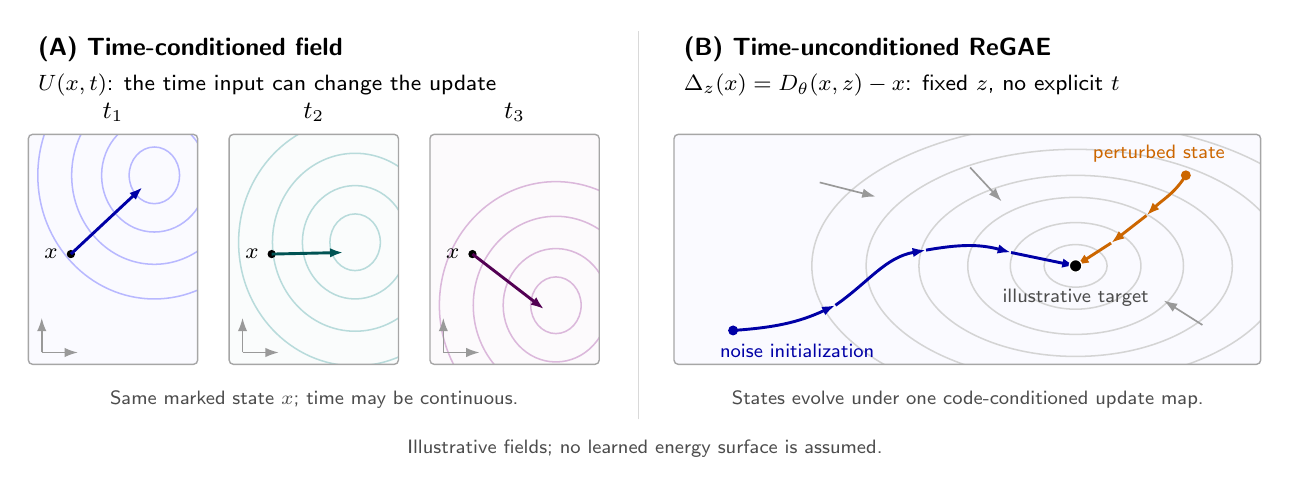
\begin{tikzpicture}[
  x=1cm,y=1cm,font=\sffamily\footnotesize,
  >={Latex[length=1.7mm,width=1.2mm]},
  frame/.style={draw=black!35,line width=.5pt,rounded corners=1.5pt},
  contour/.style={draw=black!17,line width=.55pt},
  field/.style={->,draw=black!40,line width=.6pt},
  update/.style={->,line width=1.05pt},
  smallnote/.style={font=\sffamily\scriptsize,text=black!70,align=center}
]
\node[anchor=west,font=\sffamily\bfseries\small] at (0,5.05)
  {(A) Time-conditioned field};
\node[anchor=west] at (0,4.60)
  {$U(x,t)$: the time input can change the update};
\node[anchor=west,font=\sffamily\bfseries\small] at (8.2,5.05)
  {(B) Time-unconditioned ReGAE};
\node[anchor=west] at (8.2,4.60)
  {$\Delta_z(x)=D_{\theta}(x,z)-x$: fixed $z$, no explicit $t$};
% Each thumbnail repeats the SAME state-space domain. They are snapshots
% at selected times, not a partition of states into different noise bands.
\foreach \shift/\time/\yc/\dy/\shade in
  {0/1/2.40/.85/blue,2.55/2/1.55/.02/teal,5.10/3/.75/-.70/violet}{
  \begin{scope}[shift={(\shift,1.05)}]
    \path[fill=\shade!2] (0,0) rectangle (2.15,2.92);
    \begin{scope}
      \clip (0,0) rectangle (2.15,2.92);
      \foreach \rx/\ry in {.32/.36,.67/.72,1.05/1.13,1.48/1.57}{
        \draw[draw=\shade!28,line width=.55pt]
          (1.60,\yc) ellipse[x radius=\rx cm,y radius=\ry cm];
      }
    \end{scope}
    \draw[frame] (0,0) rectangle (2.15,2.92);
    \node[font=\sffamily\small] at (1.075,3.20) {$t_{\time}$};
    \fill[black] (.54,1.40) circle[radius=1.5pt];
    \node[anchor=east,inner sep=2pt] at (.45,1.40) {$x$};
    \draw[update,draw=\shade!65!black]
      (.54,1.40)--(1.45,{1.40+\dy});
    % Identical coordinate indicators reinforce the common domain.
    \draw[field] (.17,.15)--(.63,.15);
    \draw[field] (.17,.15)--(.17,.59);
  \end{scope}
}
\node[smallnote] at (3.63,.60)
  {Same marked state $x$; time may be continuous.};
\draw[black!15,line width=.5pt] (7.75,.35)--(7.75,5.28);
% A single fixed code-conditioned state-update map. Contours are illustrative
% guides only; they do not imply that the map is an energy gradient.
\path[fill=blue!2] (8.2,1.05) rectangle (15.65,3.97);
\begin{scope}
  \clip (8.2,1.05) rectangle (15.65,3.97);
  \foreach \rx/\ry in {.40/.27,.83/.55,1.37/.87,1.99/1.15,2.66/1.48,3.35/1.82}{
    \draw[contour] (13.30,2.30) ellipse[x radius=\rx cm,y radius=\ry cm];
  }
  \draw[field] (10.05,3.36)--(10.76,3.18);
  \draw[field] (11.96,3.55)--(12.36,3.12);
  \draw[field] (14.91,1.55)--(14.42,1.86);
\end{scope}
\draw[frame] (8.2,1.05) rectangle (15.65,3.97);
% Two hand-constructed trajectories, with arrows marking repeated updates.
\draw[update,draw=blue!65!black] (8.95,1.48) to[out=4,in=205] (10.25,1.80);
\draw[update,draw=blue!65!black] (10.25,1.80) to[out=35,in=190] (11.40,2.50);
\draw[update,draw=blue!65!black] (11.40,2.50) to[out=10,in=165] (12.48,2.47);
\draw[update,draw=blue!65!black] (12.48,2.47)--(13.30,2.30);
\fill[blue!65!black] (8.95,1.48) circle[radius=1.8pt];
\node[smallnote,anchor=west,text=blue!65!black] at (8.66,1.22)
  {noise initialization};
\draw[update,draw=orange!80!black] (14.70,3.45) to[out=238,in=45] (14.20,2.94);
\draw[update,draw=orange!80!black] (14.20,2.94)--(13.75,2.59);
\draw[update,draw=orange!80!black] (13.75,2.59)--(13.30,2.30);
\fill[orange!80!black] (14.70,3.45) circle[radius=1.8pt];
\node[smallnote,anchor=east,text=orange!80!black] at (15.32,3.73)
  {perturbed state};
\filldraw[fill=black,draw=white,line width=.5pt]
  (13.30,2.30) circle[radius=2.3pt];
\node[smallnote,anchor=north] at (13.30,2.13)
  {illustrative target};
\node[smallnote] at (11.93,.60)
  {States evolve under one code-conditioned update map.};
\node[smallnote] at (7.83,-.02)
  {Illustrative fields; no learned energy surface is assumed.};
\end{tikzpicture}

  \caption{Conceptual comparison of time dependence. (A) Selected times index fields over the same state coordinates; the marked state can receive different updates. The panels are time slices, not disjoint regions of state space. (B) A fixed-code ReGAE uses one induced displacement field for both noise initialization and a perturbed state. The contours and paths are constructed illustrations, not measured trajectories, learned energies, or evidence of convergence. The comparison concerns the learned operator; an external sampling schedule can still introduce time dependence.}
  \label{fig:time-fields}
\end{figure*}

The basin interpretation is useful when a desired reconstruction is an attracting fixed point. It is not a consequence of omitting a clock. A learned vector field need not be the gradient of any scalar energy, and generative transport need not minimize an objective until reaching a stationary state. In particular, a diffusion or flow trajectory's terminal sample need not be an equilibrium of its field. For ReGAE, local contraction would be a sufficient mechanism for repair; Appendix~\ref{sec:geometry-notes} states that condition and an explicit Euler connection as mathematical interpretations, not measured properties.

The distinction between the neural map and the whole sampler also matters. The saved Pandora video routine varies its injected noise with frame index and averages overlapping predictions. Its denoisers do not receive that index, but the resulting stochastic canvas update still depends on time through the external schedule. Moreover, the shifted Gencoder target encourages progression between views, so its intended behavior is not convergence to a single unchanging image.

\subsection{Modeling representations with the same kind of model}

A ReGAE can model a dataset's samples, and another ReGAE can model the resulting representations. Reusing the denoiser family at both levels expresses a hypothesis that reconstruction is a useful operation across different levels of abstraction. The higher level need not be spatial: it should model whatever structure is meaningful in its input representations.

This motivates recursive or fractal organizations of models. The present experiment instantiates two separately trained members of the family, without sharing their weights. It models an encoder's output fields, not the lower model's complete internal computation or learning algorithm. Architectural reuse thus provides a concrete starting point for that broader motivation; it does not by itself demonstrate meta-learning, self-modeling, or general intelligence. The number of levels and the relationships learned at each remain design questions.

\subsection{Learning and compression}
\label{sec:compression}

The memorization question can be restated as a question about where dataset information is stored. Shared parameters describe regularities that recur across samples; individual latent tensors describe sample-specific variation. A further model can learn regularities among those tensors, reducing the relational information that must be supplied explicitly when generating plausible data. In Pandora's Cluster, that information includes spatial organization. In another dataset, it could concern a different distribution or relationship.

This is a representational compression argument, not yet a claim about a complete image codec. A small code must be interpreted together with the model that decodes it, its numerical precision, and the fidelity of reconstruction. For the present configuration, 3,072 RGB channel values become 256 latent scalars. The factor of 12 in scalar count becomes a factor of three when comparing 8-bit RGB with 32-bit latent values, before including network storage. Appendix~\ref{sec:storage} provides the corresponding payload accounting.

A minimum-description-length view includes both model and data terms~\cite{mdl}. A practical codec additionally needs a coding procedure and a rate--distortion evaluation~\cite{coin}. Learning a generator over codes does not prove that the exact original code arrangement can be discarded without loss. ReGAE provides a concrete setting for studying successive levels of regularity, while the broader intelligence-as-compression interpretation remains a subject for a companion essay.

\subsection{Multiplicative gain in the default implementation}

The denoiser used in the proof of concept includes a multiplicative feature branch called \emph{gravity}. It amplifies or attenuates features through a learned gain; the term is an analogy, not a physical law or a requirement of the ReGAE family. The earlier exponential gate allowed unbounded gain. The author recalls stars becoming progressively brighter followed by dark regions, described as \emph{neural black holes}. The associated recordings and checkpoints were not retained.

An isolated gate-only recurrence $h_{t+1}=h_t\exp(g_t)$ accumulates gain as $h_T=h_0\exp(\sum_{t<T}g_t)$, illustrating a possible amplification mechanism. This does not establish the cause of the reported darkening or imply an implemented reset rule. The later bounded activation caps this individual gain. It does not prove stability of the full recurrent network. The precise gate and its placement are documented with the application architecture in Appendix~\ref{sec:implementation}.

\subsection{Scope and next steps}

The general design accommodates conditional and unconditional modeling of one-, two-, or three-dimensional data; the evidence presented here concerns one two-dimensional visual proof of concept. Controlled regeneration measurements, architecture and loss comparisons, and applications to other data types are not part of the current report. One-step denoising training also does not explicitly optimize long-horizon behavior.

The next revision can strengthen the presentation using the existing stills, videos, checkpoints, and run records. No new experiment is required to make the family definition and the reported application precise. Further empirical evaluation can test how broadly the regenerative operator transfers across data representations, which properties are retained at each level, and how reliably perturbations are repaired.


\section{Conclusion}
ReGAE separates learning local appearance from learning the spatial organization of the resulting representations. Its central mechanism is a denoising predictor over spatial latent windows whose targets correspond to fractionally displaced image patches. Reusing the denoiser architecture across levels supports a simple hierarchical construction, and overlapping recurrent sampling turns the learned transition into a procedure for image generation and traversal. The archived implementation and training traces establish a concrete starting point for studying this construction. Its reported long-range visual behavior remains qualitative, and neither faithful navigation nor stable recurrence follows from the one-step objectives alone. The broader opportunity is to study how reusable reconstruction operators can organize information at successively larger scales, with explicit attention to the distinction between reconstructing stored structure and generating plausible alternatives.

\paragraph{Data and code.}
The original notebooks and manuscript sources are available in the \href{https://github.com/magnux/neural_pandoras_cluster}{Neural Pandora's Cluster repository}. The source image is credited to NASA, ESA, CSA, Ivo Labbe (Swinburne), and Rachel Bezanson (University of Pittsburgh), with image processing by Alyssa Pagan (STScI)~\cite{webb}. The experiments use the rendered image as a visual learning problem; generated outputs are not astronomical observations.

{\small
\bibliographystyle{ieeenat_fullname}
\bibliography{references}
}

\clearpage
\appendix
\section{Archive and Implementation Details}
\label{sec:archive}

\paragraph{Source of the technical description.}
The principal implementation is the v2 notebook, while v0 documents architectural and sampling development. The repository preserves both original files in its notebooks directory, together with their SHA-256 hashes. The description in this manuscript was obtained by inspecting code and saved outputs. No notebook training or generation cell was executed to prepare this draft. The separate NVD notebooks are not evidence for the ReGAE results.

\paragraph{Stage boundaries.}
The v2 configuration jointly trains the image encoder and decoder, then constructs latent maps for the Gencoder. The latter is a separately trained instance of the decoder family with 256 input/output channels and no external conditioning code. The image decoder uses three input/output channels and latent conditioning. Shared architecture thus refers to the computational construction, not tied weights. The patch-relative positional parameters do not encode global source-image coordinates.

\paragraph{Optimization and reproducibility.}
The recorded environment reports PyTorch 2.2.2 with CUDA 12.1, and the code sets a random seed of 4202. These facts do not specify the original GPU, elapsed training time, or complete software environment. The archive contains configured training loops and saved displays, but no complete execution log establishing every historical state. In v2, the Gencoder loop computes a decaying learning rate but assigns it to the AE optimizer, leaving the Gencoder optimizer unchanged by that schedule. This is preserved as a historical qualification rather than silently corrected. Exact reproduction should distinguish a faithful historical configuration from a cleaned implementation.

\paragraph{Exploratory sampling in v0.}
The earlier notebook includes source-code reconstruction, latent generation, random overlapping patch updates, repeated local refinement, and shifted raster sweeps. Some updates protect previously completed pixels or use update-budget masks. Their motivation includes an analogy to wave-function-collapse-style synthesis. The cells do not implement a documented entropy-ranked constraint-propagation algorithm, and their current channel and conditioning assumptions are not mutually consistent with all retained network definitions. We therefore avoid presenting them as a verified benchmark of sampling strategies. The later v2 synchronous overlap average is specified explicitly in Eq.~\eqref{eq:regae-overlap-update}.

\paragraph{Extent of a latent window.}
The decoder tiles $32\times32$ generated image patches into a $1024\times1024$ macro-image. The source crops used to build a corresponding training window are positioned by the rounded lattice in Eq.~\eqref{eq:regae-grid-origins}, rather than exactly 32 pixels apart. ``Megapixel window'' consequently describes the decoded tile extent; it does not assert that all sampled training windows form an exact, gap-free partition of the source image.

\paragraph{Visual evidence to add from existing runs.}
The most informative additions would be a source region alongside its patch-code reconstruction, a spatially coherent Gencoder sample, and a short sequence showing a typical trajectory and a reported jump. Each should identify its checkpoint, sampler configuration, and whether its RGB rendering uses fresh noise. The unstable exponential-gate example cannot currently be illustrated from an original recording and should remain identified as an anecdote. This list specifies documentation needs, not new experiments or figures that already exist in this draft.

\section{Storage Accounting for the Proof of Concept}
\label{sec:storage}

The stored parameter counts are 4,673,752 for the encoder, 50,986,296 for the conditional image denoiser, and 85,479,680 for the Gencoder. These counts describe this implementation, not a required model size. Table~\ref{tab:storage} calculates uncompressed payloads in decimal megabytes. A code grid alone does not specify a complete codec for the image, including its boundary conventions and reconstruction distortion.

\begin{table}[t]
  \centering
  \small
  \setlength{\tabcolsep}{5pt}
  \begin{tabular}{lr}
    \toprule
    Representation or parameter payload & MB \\
    \midrule
    Source RGB array, 8 bits per channel & 710.45 \\
    One $419\times551\times256$ grid, FP32 & 236.41 \\
    Image encoder and denoiser, FP32 & 222.64 \\
    Gencoder, FP32 & 341.92 \\
    Image denoiser plus one grid, FP32 & 440.36 \\
    AE and Gencoder parameters, FP32 & 564.56 \\
    \bottomrule
  \end{tabular}
  \caption{Calculated uncompressed payloads for the Pandora setup. Rows describe different accounting choices, not interchangeable complete codecs. Optimizer state and file overhead are excluded. The four shifted training grids occupy approximately 945.64 MB in FP32.}
  \label{tab:storage}
\end{table}

AMSGrad stores three moment-related tensors per parameter in addition to the weights. Including these tensors in FP32 can bring training checkpoints near the author's recalled 0.89 GB for the AE and 1.4 GB for the Gencoder. This is an inference from the optimizer and parameter counts, not a measurement of the unavailable checkpoint files. A storage comparison with JPEG or another codec would also need quantization, coding, model costs, and matched reconstruction distortion.

\section{Preserved Training Plots}
\label{sec:traces}
The plots reproduce unchanged PNGs from the archived v2 outputs. Their horizontal axes count optimizer updates despite the inherited ``epoch'' label. Vertical values are square roots of different training objectives and are not directly comparable.

\begin{figure*}[t]
  \centering
  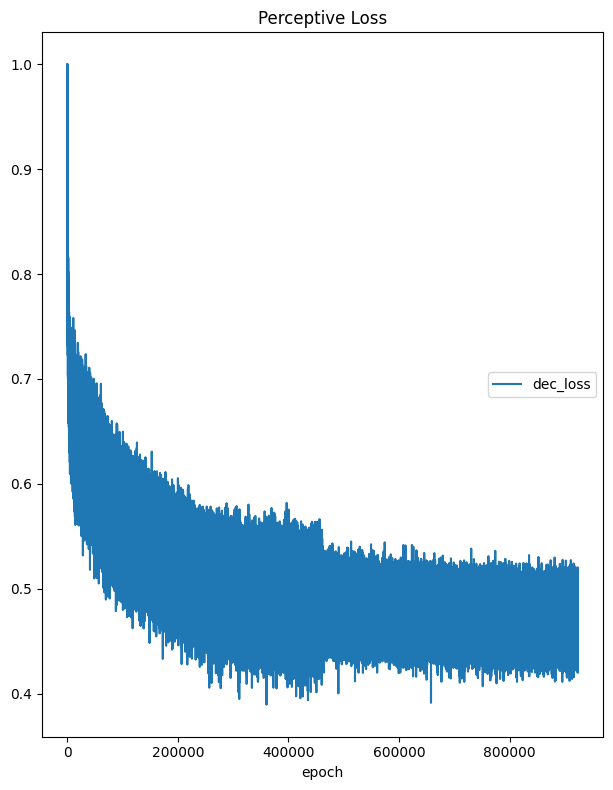
\includegraphics[width=0.86\textwidth]{figures/ae-training.png}
  \caption{Saved image-autoencoder training display (v2, code cell 39 under zero-based notebook indexing). The summary reports minimum 0.389, current 0.450, and maximum 1.000; the history was clipped to $[0,1]$ for plotting. The displayed quantity is the square root of the VGG feature $L_1$ loss. The history supports optimization of the training objective, not a held-out quality estimate.}
  \label{fig:ae-trace}
\end{figure*}

\begin{figure*}[t]
  \centering
  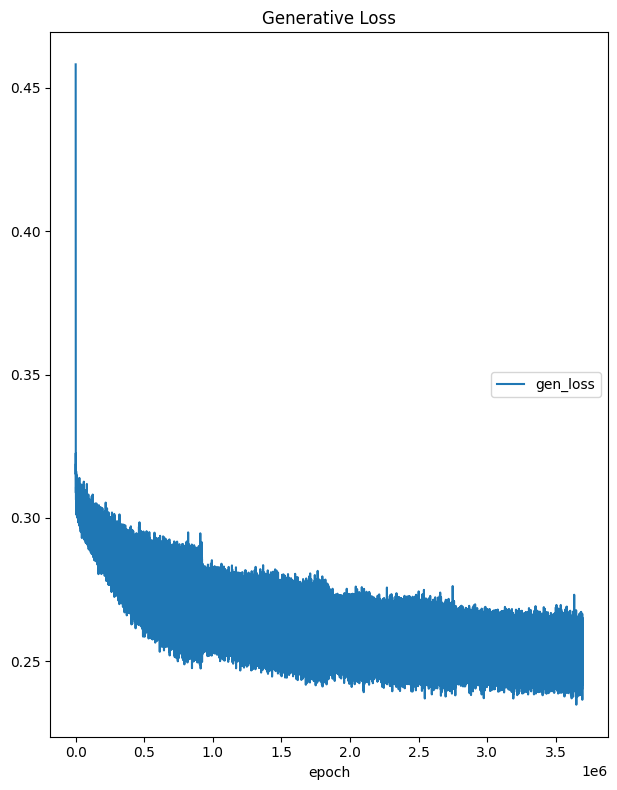
\includegraphics[width=0.86\textwidth]{figures/gencoder-training.png}
  \caption{Saved Gencoder training display (v2, code cell 46 under zero-based notebook indexing). The summary reports minimum 0.235, current 0.252, and maximum 0.458. The displayed quantity is the square root of the latent $L_1$ prediction loss. No new training was run to produce this figure.}
  \label{fig:gencoder-trace}
\end{figure*}

\end{document}
